\documentclass[11pt]{article}

\usepackage[utf8]{inputenc}
\usepackage[T1]{fontenc}
\usepackage{lmodern}
\usepackage[a4paper,margin=1in]{geometry}
\usepackage{amsmath}
\usepackage{graphicx}
\usepackage{booktabs}
\usepackage{siunitx}
\usepackage{microtype}
\usepackage[round]{natbib}
\bibliographystyle{plainnat}
\usepackage[hidelinks]{hyperref}

\sisetup{detect-weight=true, detect-family=true}

\title{\textbf{W/kg on a Climb is a Distribution, not a Verdict:\\
Estimating Cycling Climbing Power with Honest Uncertainty}}

\author{Carlo Vilches\thanks{Corresponding author.
Email: \texttt{cvilchce15@alumnes.ub.edu}}\\[2pt]
\normalsize Universitat de Barcelona, Barcelona}
\date{2026}

\begin{document}

\maketitle

\begin{abstract}
\noindent
Every Grand Tour mountain stage now ends the same way: a self-appointed
``watts watcher'' posts a single relative-power figure --- ``\num{6.4}~W/kg'' ---
and declares the rider a mutant. The point estimate is the problem. The inputs
that feed it (rider mass, frontal area, rolling resistance, wind, air density,
the timing pulled from television) are not known precisely, so a number quoted
to two decimals is false precision dressed as evidence. We describe a small,
reproducible estimator that keeps the physics honest about what it does not
know. A validated power-balance model \citep{martin1998} converts public climb
data (length, elevation gain, time) into mechanical power, and a Monte Carlo
layer propagates the uncertainty in every uncertain input into a
\emph{distribution} of W/kg rather than a single value. The output is a median,
a 90\% credible interval, and the probability of exceeding a chosen
physiological threshold. On the demonstration climb (Alpe d'Huez, \num{40}:00)
the estimate is \num{5.77}~W/kg (90\% CI \numrange{5.38}{6.33}),
$P(>\!6.2)=\SI{9.5}{\percent}$. Applied to two iconic Pyrenean efforts, the
method places Froome (Ax~3~Domaines, 2013) at a median \num{6.35}~W/kg
(\numrange{5.86}{7.05}, $P(>\!6.2)=\SI{67}{\percent}$) --- straddling the
informal ``suspicion'' line, genuinely ambiguous --- and Pogačar (Plateau de
Beille, 2024) at \num{7.00}~W/kg (\numrange{6.46}{7.77},
$P(>\!6.2)=\SI{100}{\percent}$) --- unambiguously above the old ceiling. The
method is deliberately one of \emph{estimation, not accusation}: the model is
sound, the inputs are uncertain, and so the result is reported as a range. ``Above the old ceiling'' is not ``doping.''
\end{abstract}

\section{Introduction}

Relative power output --- watts per kilogram of body mass --- has become the
de~facto lie detector of professional cycling. On a sustained climb, where
aerodynamic drag is small and gravity dominates, W/kg is closely tied to ascent
rate, so a fast climb invites an immediate back-of-envelope estimate and, with
it, a verdict. The cultural ritual is familiar: a stage finishes, an estimate
circulates, and a figure crosses some remembered ``ceiling'' for clean
performance, at which point suspicion is treated as established fact.

There are two distinct problems with this ritual, and only one of them is about
doping. The first is that a single point estimate misrepresents the evidence.
The quantities required to turn a climb into a power figure are not measured ---
they are guessed, and some are guessed badly. Published rider weights are
unreliable and mass is the single largest lever on the estimate; wind and
drafting are usually unknown; the climb's exact length, gradient and the rider's
finishing time are read off television graphics or third-party segments. A
figure quoted as ``\num{6.4}~W/kg'' hides all of this behind a decimal point it
has not earned.

The second problem is the standard used to interpret the figure. The most widely
circulated shortcut is the VAM rule (vertical ascent metres per hour divided by a
gradient-dependent factor), popularised as the ``Ferrari factor.'' It is a
coaching heuristic, not a peer-reviewed model, and it was never intended to
adjudicate guilt. The rigorous alternative has existed since 1998:
\citet{martin1998} derived and experimentally validated a mathematical model of
road-cycling power, finding modelled and measured power highly correlated
($R^2=0.97$) and not statistically different, with a standard error of estimate
of only \SI{2.7}{\watt}. That model --- gravity, rolling resistance, aerodynamic
drag and drivetrain losses --- is the defensible backbone for any W/kg estimate.

This paper takes the position that the physics is the easy part and the honesty
is the hard part. We pair the validated power-balance model with explicit
uncertainty propagation, so that the output is never a single number but a
distribution: a median, a 90\% credible interval, and an exceedance probability
$P(\text{W/kg}>\tau)$ for a user-chosen threshold $\tau$. We situate the result
in the power--duration framework of the Record Power Profile
\citep{pinot2011}, which treats sustainable power as a function of effort
duration rather than a single scalar. The aim throughout is to estimate a
mechanical effort \emph{with} its uncertainty, and to refuse the leap from ``above
the old ceiling'' to ``cheating.''

\section{Methods}

\subsection{The physical power--balance model}

For a rider of total system mass $m$ (rider plus bicycle and kit) ascending a
road of gradient $\theta$ at ground speed $v$, the steady-state mechanical power
delivered at the rider is the sum of the power to lift the system against
gravity, to overcome rolling resistance, and to push air aside, divided by
drivetrain efficiency $\eta$:
\begin{equation}
P \;=\; \frac{1}{\eta}\Big[\,
\underbrace{m\,g\,\sin\theta\;v}_{\text{gravity}} \;+\;
\underbrace{C_{rr}\,m\,g\,\cos\theta\;v}_{\text{rolling}} \;+\;
\underbrace{\tfrac{1}{2}\,\rho\,C_dA\,(v+v_{w})^{2}\,v}_{\text{aerodynamic}}
\,\Big],
\label{eq:power}
\end{equation}
where $g=\SI{9.81}{\meter\per\second\squared}$, $\rho$ is air density, $C_dA$ the
effective drag area, $C_{rr}$ the rolling-resistance coefficient and $v_w$ a
headwind component ($v_w>0$ is a headwind). Equation~\eqref{eq:power} is the
form validated by \citet{martin1998}; on a steep climb the gravity term
dominates, but the rolling and aerodynamic terms remain non-negligible and are
retained. Relative power is $P/m_{\text{rider}}$, reported per kilogram of rider
body mass.

\subsection{Three estimators, from crude to defensible}

The implementation exposes three estimators that share the same public inputs
--- climb length $L$, elevation gain $\Delta h$, time $t$ and an assumed rider
mass --- and differ in rigour.

\paragraph{(i) Ferrari / VAM heuristic.}
The social-media shortcut. With $\mathrm{VAM}=\Delta h\cdot 3600/t$ (vertical
metres per hour) and a gradient $s$ in percent,
\begin{equation}
\text{W/kg}_{\text{Ferrari}} \;=\; \frac{\mathrm{VAM}}{(2 + s/10)\cdot 100}.
\end{equation}
It is fast, requires no assumptions about mass or drag, and is explicitly
labelled an approximation: a coaching rule of thumb, \emph{not} a peer-reviewed
estimator. We report it only to show how close --- or how far --- the crude
heuristic lands relative to the physical model.

\paragraph{(ii) Physical point estimate.}
Equation~\eqref{eq:power} evaluated once at central values of every parameter
($m_{\text{bike}}=\SI{8.0}{\kg}$, $\rho=\SI{1.10}{\kg\per\meter\cubed}$,
$C_dA=\SI{0.32}{\meter\squared}$, $C_{rr}=0.004$, $v_w=0$, $\eta=0.976$),
with road speed $v=L/t$ and gradient inferred from $L$ and $\Delta h$. This is
the best single number the physics can give --- and precisely the number we
argue should never be reported alone.

\paragraph{(iii) Monte Carlo distribution.}
The estimator we advocate. Rather than evaluating Equation~\eqref{eq:power} at
fixed inputs, we draw $n=\num{200000}$ samples for every uncertain quantity from
independent priors (Table~\ref{tab:priors}), evaluate the model for each draw,
and report the resulting distribution of W/kg by its median, its 5th and 95th
percentiles (a 90\% credible interval), and the exceedance probability
$P(\text{W/kg}>\tau)$.

\subsection{Uncertainty propagation and priors}

\begin{table}[t]
\centering
\caption{Monte Carlo priors. Each uncertain input is drawn from a normal
distribution; a single \texttt{unc\_scale} multiplier widens or narrows every
standard deviation together (defaults shown). The mass terms carry by far the
largest standard deviation relative to their effect on the estimate, which is
why mass is the dominant lever.}
\label{tab:priors}
\begin{tabular}{@{}llll@{}}
\toprule
Input & Symbol & Mean & Std.\ dev.\ (default) \\
\midrule
Rider mass        & $m_{\text{rider}}$ & published value & \SI{2.0}{\kg} \\
Bike + kit mass   & $m_{\text{bike}}$  & \SI{8.0}{\kg}   & \SI{0.5}{\kg} \\
Air density       & $\rho$             & \SI{1.10}{\kg\per\meter\cubed} & \num{0.04} \\
Drag area         & $C_dA$             & \SI{0.32}{\meter\squared} & \num{0.03} \\
Rolling coeff.    & $C_{rr}$           & \num{0.004}     & \num{0.0006} \\
Wind component    & $v_{w}$            & \SI{0.0}{\meter\per\second} & \SI{1.5}{\meter\per\second} \\
Drivetrain eff.   & $\eta$             & \num{0.976}     & \num{0.005} \\
Elevation gain    & $\Delta h$         & measured        & 2\% of $\Delta h$ (DEM/GPS) \\
Climb length      & $L$                & measured        & 1\% of $L$ \\
\bottomrule
\end{tabular}
\end{table}

The priors in Table~\ref{tab:priors} encode where the ignorance actually lives.
Rider mass is given a \SI{2}{\kg} standard deviation because published racing
weights are systematically unreliable, and because mass enters
Equation~\eqref{eq:power} both in the numerator (the system being lifted) and in
the denominator (the body mass we divide by); it is the single largest source of
spread in the output. Wind is given a \SI{1.5}{\meter\per\second} standard
deviation centred on zero, reflecting that the true head/tail component on a
televised climb is essentially unknown and matters most on shallower gradients.
Air density, drag area, rolling resistance and drivetrain efficiency carry
narrower, physically motivated priors. Geometry (length and gain) is given small
multiplicative noise to represent DEM and GPS error. The priors are deliberately
wide and editable in one line of code; a single \texttt{unc\_scale} multiplier
scales every standard deviation at once, so a reader who believes the inputs are
better (or worse) constrained can widen or narrow the whole interval coherently.

\subsection{Power--duration context}
\label{sec:pdcontext}

A W/kg figure is meaningless without a duration attached: \num{7}~W/kg for one
minute and for forty minutes describe entirely different physiological feats. We
therefore interpret each estimate within the Record Power Profile framework of
\citet{pinot2011}, in which sustainable power follows an approximately hyperbolic
relationship with effort duration and the profile across durations acts as a
``signature'' of a rider's physical capacity. Every estimate in this paper is a
sustained climbing effort of roughly \numrange{20}{40} minutes, and should be
read as a point on that duration curve, not as a context-free scalar.

\section{Results}

All numbers below are produced directly by the accompanying code
(\texttt{wkg\_estimator.py} and \texttt{compare\_climbs.py}); the figures are the
unmodified outputs of those scripts.

\subsection{Demonstration: Alpe d'Huez}

The demonstration applies all three estimators to a canonical effort: Alpe
d'Huez, \SI{13.2}{\km} at \SI{8.1}{\percent}, climbed in \num{40}:00 by a
\SI{64}{\kg} rider (VAM \SI{1606}{\meter\per\hour}). The Ferrari heuristic returns
\num{5.71}~W/kg and the physical point estimate \num{5.76}~W/kg --- reassuringly
close, confirming the crude rule lands near the validated model for a typical
climbing gradient. The Monte Carlo layer turns this into a distribution
(Figure~\ref{fig:demo}): median \num{5.77}~W/kg, 90\% credible interval
\numrange{5.38}{6.33}, and $P(\text{W/kg}>6.2)=\SI{9.5}{\percent}$. The single
number and the distribution agree on the centre; only the distribution also tells
you that, given honest input uncertainty, this effort sits comfortably below the
\num{6.2} line about nine times out of ten.

\begin{figure}[t]
\centering
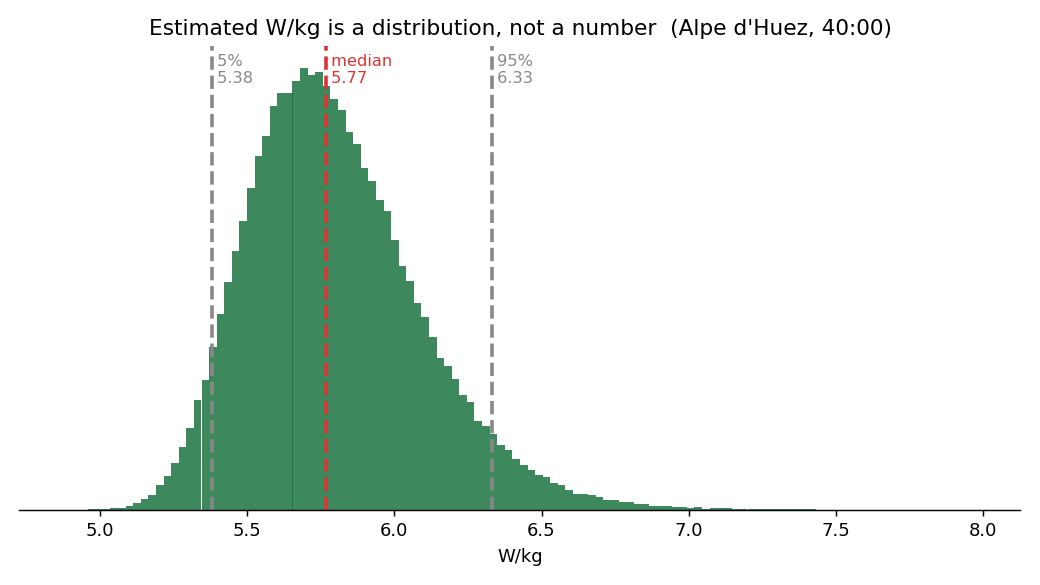
\includegraphics[width=0.92\textwidth]{wkg_distribution.png}
\caption{The estimate is a distribution, not a number. Monte Carlo output for
the Alpe d'Huez demonstration: median \num{5.77}~W/kg with a 90\% credible
interval of \numrange{5.38}{6.33}~W/kg. The point estimate (\num{5.76}~W/kg)
locates the centre; the spread is the honest part.}
\label{fig:demo}
\end{figure}

\subsection{Two Pyrenean efforts, eleven years apart}

The substantive comparison runs the same pipeline on two famous climbs separated
by more than a decade (Table~\ref{tab:results}, Figure~\ref{fig:compare}). Both
were widely cited at the time as ``too fast to be clean,'' and the method lets us
ask whether that label is supported by the evidence \emph{once the uncertainty is
made explicit}.

\begin{table}[t]
\centering
\caption{Estimator outputs for the two climbs, as printed by
\texttt{compare\_climbs.py}. The Monte Carlo column is the result we advocate
reporting; the single-figure columns are shown only for comparison. The
suspicion threshold is $\tau=\num{6.2}$~W/kg.}
\label{tab:results}
\begin{tabular}{@{}lcc@{}}
\toprule
& \textbf{Froome} & \textbf{Pogačar} \\
& Ax~3~Domaines (2013) & Plateau de Beille (2024) \\
\midrule
Climb length            & \SI{8.9}{\km}  & \SI{15.8}{\km} \\
Gradient                & \SI{7.48}{\percent} & \SI{7.93}{\percent} \\
Time                    & \num{23}:14 & \num{39}:43 \\
VAM                     & \SI{1715}{\meter\per\hour} & \SI{1887}{\meter\per\hour} \\
Assumed mass            & \SI{67}{\kg} & \SI{66}{\kg} \\
\midrule
Ferrari (heuristic)     & \num{6.24} & \num{6.76} \\
Physical (point)        & \num{6.35} & \num{7.00} \\
\textbf{MC median}      & \textbf{\num{6.35}} & \textbf{\num{7.00}} \\
\quad 90\% CI           & \numrange{5.86}{7.05} & \numrange{6.46}{7.77} \\
\quad $P(>\!6.2)$       & \SI{67}{\percent} & \SI{100}{\percent} \\
\bottomrule
\end{tabular}
\end{table}

\begin{figure}[t]
\centering
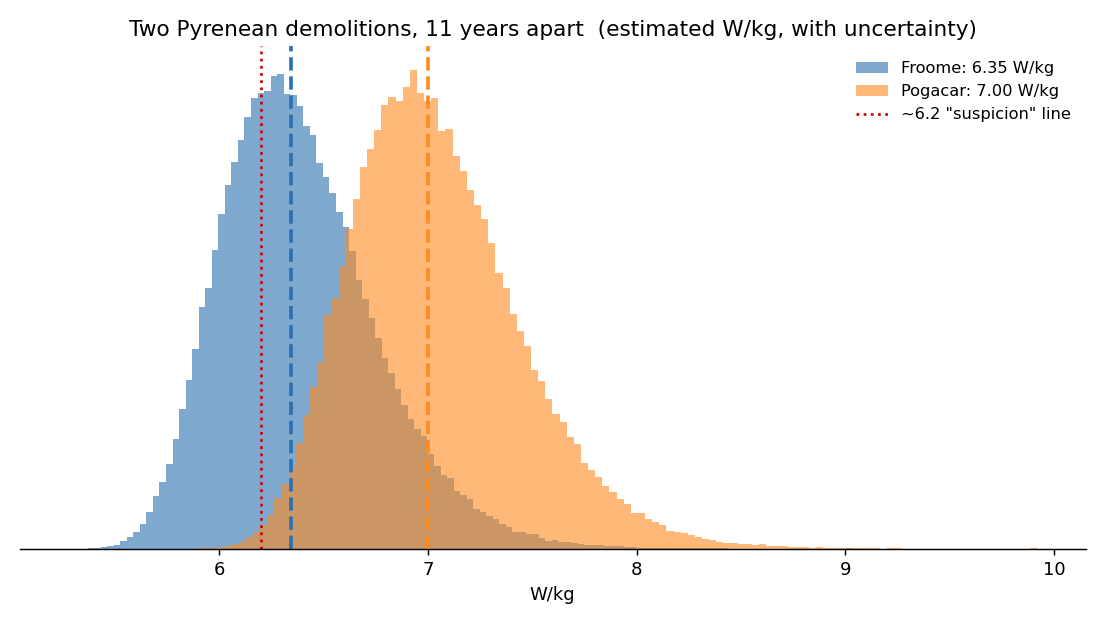
\includegraphics[width=0.95\textwidth]{froome_vs_pogacar.png}
\caption{Two Pyrenean efforts, eleven years apart, with their full estimated
W/kg distributions. Froome's distribution (median \num{6.35}~W/kg) straddles the
informal \num{6.2} suspicion line (dotted); Pogačar's (median \num{7.00}~W/kg)
sits entirely to its right. The overlap on the left tells the whole story: one
effort is ambiguous, the other is not.}
\label{fig:compare}
\end{figure}

The two cases land very differently. Froome's 2013 Ax~3~Domaines effort estimates
to a median of \num{6.35}~W/kg with a 90\% interval of \numrange{5.86}{7.05} and
$P(\text{W/kg}>6.2)=\SI{67}{\percent}$. The distribution \emph{straddles} the
\num{6.2} line: roughly a third of the credible interval lies below it. This is
the quantitative shape of a genuinely ambiguous case --- which is precisely why
the effort was argued about, inconclusively, for years. A point estimate of
\num{6.35} reads like an indictment; the interval reveals that the evidence does
not actually clear the line with confidence.

Pogačar's 2024 Plateau de Beille effort is different in kind. The median is
\num{7.00}~W/kg, the 90\% interval is \numrange{6.46}{7.77}, and
$P(\text{W/kg}>6.2)=\SI{100}{\percent}$: \emph{every} sample in the credible
interval clears the suspicion line, and does so over a climb more than twice as
long. Here the uncertainty does not rescue ambiguity --- the entire distribution
sits above the old ceiling. The same method, applied to two efforts eleven years
apart, separates ``on the line'' from ``clearly past it'' without ever collapsing
either into a single accusatory figure.

We stress what this does and does not say. It says that, conditional on the
public data and the priors in Table~\ref{tab:priors}, Pogačar's mechanical W/kg
on that climb almost certainly exceeded \num{6.2} and Froome's plausibly did not.
It does not say either rider was or was not doping. The \num{6.2} line is a
remembered heuristic ceiling, not a biological constant, and the ceiling itself
can move (Section~\ref{sec:discussion}).

\section{Discussion and Limitations}
\label{sec:discussion}

The estimator is honest about its own scope, and the limitations are not
footnotes --- they are the point.

\subsection{Why the two estimates are not comparable}
\label{sec:context}

The model estimates the mechanical power of one effort, and nothing more. It does
not say whether a given W/kg is physiologically remarkable, and --- more to the
point here --- it does not place two efforts on a common axis. Reading Froome's
\num{6.35} and Pogačar's \num{7.00} as two measurements of the same quantity is a
category error, for two independent reasons: the efforts differ in duration, and
they were ridden in different race contexts. Both differences block a like-for-like
reading, and they cut in both directions rather than toward a verdict.

\paragraph{Duration: the clean axis.}
The least disputable difference is simply how long each power was held: Froome's
effort lasted about \num{23} minutes, Pogačar's nearly \num{40}. By the
power--duration relationship of \citet{pinot2011} --- the same Record Power
Profile framework introduced in Section~\ref{sec:pdcontext} --- sustainable power
declines as duration grows, so a higher W/kg held for almost twice as long is a
strictly harder point on the curve, independent of any assumption about the rider,
the weather or the race. This is enough on its own: \num{7.00}~W/kg for \num{40}
minutes and \num{6.35}~W/kg for \num{23} minutes are not ``\num{0.65} apart'' in
any physiologically meaningful sense, because they sit at different places on the
duration curve. The raw subtraction that fuels social-media comparisons is the
error this axis exposes.

\paragraph{Race context: a filter that cuts both ways.}
The second difference is the race situation, and here the literature counsels
caution, not a conclusion. Climbing power is conditioned by accumulated load
\citep{leo2022}, by gradient \citep{valenzuela2022} and by stage type
\citep{sanders2021}, so the surrounding conditions change what a number means ---
in either direction. The two efforts sat very differently on these axes. Froome's
came in the opening week, on low cumulative race load; but within that stage it
followed an earlier hors-cat\'egorie climb (the Col de Pailh\`eres) and was
decided by roughly \SI{5}{\km} alone at full effort, so it was neither a
fully fresh nor a steady-state test. Pogačar's came at the end of the second week,
closing a long mountain stage of roughly \SI{5000}{\meter} of climbing in heat.
These facts --- drawn from the public race record and kept separate from the model
outputs --- do not establish that either effort was the greater feat; they
establish that the two were produced under conditions different enough that the
medians should not be stacked side by side. The honest use of context is to block
the false comparison, not to extract a new verdict from it.

Read together, the two cases make the same point about a \emph{pair} of estimates
that the rest of the paper makes about a \emph{single} one: a W/kg figure is not
self-interpreting, and two figures are no more comparable than one is conclusive.
Different durations and different race contexts mean the numbers are not on one
scale --- which is a reason to resist the comparison, in both directions, not a
lever for deciding whose climb was more extraordinary or whose was more suspect.

\subsection{Scope and limitations}

\paragraph{There is no fatigue layer.}
Most importantly, the model has no representation of accumulated fatigue, heat,
nutrition or stage context. It estimates mechanical power, full stop --- it does
not judge whether that power is ``clean.'' This is a deliberate boundary: adding
a physiological-plausibility layer would re-introduce exactly the accusatory leap
the method is built to avoid. ``Above the old ceiling'' has many innocent
explanations (altitude acclimatisation, heat protocols, nutrition, aerodynamic
and training advances, a genuinely exceptional athlete), and the model cannot
distinguish among them.

\paragraph{Measuring performance is intrinsically noisy.}
Even the underlying quantity is stochastic. \citet{passfield2017} emphasise that
field power data have an inherently variable, stochastic nature that simple
summary figures cannot represent --- which is the empirical justification for
reporting a distribution rather than a point. Our inputs are worse than a power
meter on the bike: mass is assumed, wind is unknown, and the geometry and timing
are read off television. The credible interval is wide because the honest answer
is wide.

\paragraph{Validation is by plausibility, not case-by-case ground truth.}
We do not have the riders' true power files, so we cannot validate any single
estimate against measured power. What anchors the method to reality is published
longitudinal data such as \citet{pinot2015}, a six-year monitoring case study of
a twice top-ten Grand Tour finisher whose recorded power outputs across durations
from five minutes to four hours bound the physiological range these estimates
should fall within. Our medians for elite climbs are consistent with that range,
which is a plausibility check --- not a per-case proof.

\paragraph{Scope statement.}
In one sentence: this is a mechanical estimate of a single effort, built on a
validated power model but fed by uncertain inputs (mass, wind, television data),
with no fatigue model and no case-by-case empirical validation. Reported as a
range, it is informative; collapsed to a point and read as a verdict, it is
exactly the false precision it was written to replace.

\section{Conclusion}

The watts-watcher ritual fails not because the physics is wrong but because a
point estimate pretends to a certainty the inputs cannot support. Coupling the
validated power-balance model of \citet{martin1998} with explicit Monte Carlo
propagation replaces the single ``mutant'' figure with a median, a 90\% credible
interval, and an exceedance probability. On our two test cases that distinction
is decisive: Froome's 2013 climb straddles the suspicion line and is genuinely
ambiguous ($P(>\!6.2)=\SI{67}{\percent}$), while Pogačar's 2024 climb sits
entirely above it ($P(>\!6.2)=\SI{100}{\percent}$). The method estimates with
uncertainty; it does not accuse. The number worth reporting was never a number
--- it was a range.

\paragraph{Reproducibility.}
All results, including both figures and every value in
Tables~\ref{tab:priors}--\ref{tab:results}, are produced by the accompanying
code (\texttt{wkg\_estimator.py}, \texttt{compare\_climbs.py}) and verified by a
sanity-test suite (\texttt{python -m pytest}).

\bibliography{refs}

\end{document}
